%
% fl.tex -- focal length
%
% (c) 2018 Prof Dr Andreas Müller, Hochschule Rapperswil
%
\documentclass[tikz,12pt]{standalone}
\usepackage{times}
\usepackage{amsmath}
\usepackage{txfonts}
\usepackage[utf8]{inputenc}
\usepackage{graphics}
\usepackage{color}
\usepackage{pifont}
\usetikzlibrary{arrows,intersections,math,calc}
\begin{document}

\def\punkt#1{
        \fill[color=white] #1 circle[radius=0.08];
        \draw #1 circle[radius=0.08];
}

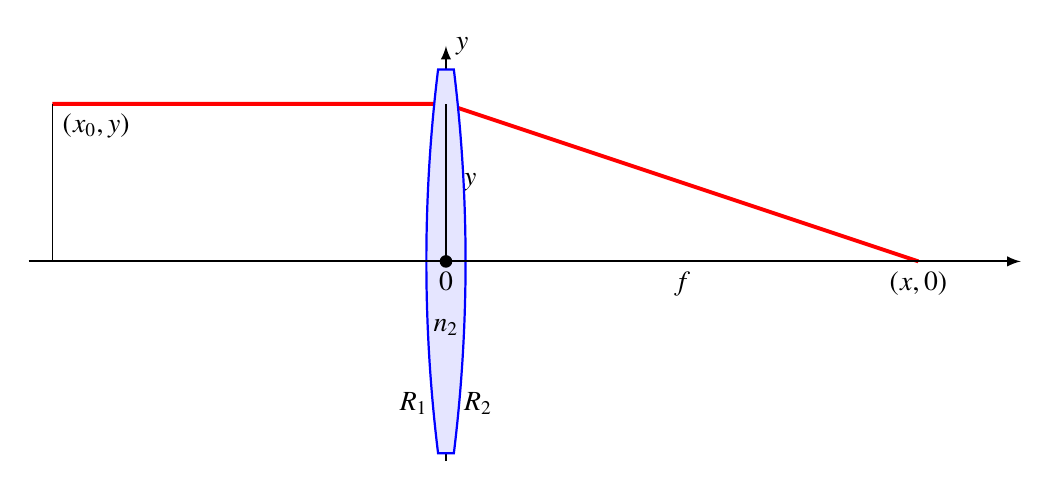
\begin{tikzpicture}[>=latex,thick]

\def\l{5}
\def\w{7}
\def\a{7}
\def\R{20}
\def\d{0.1}

\pgfmathparse{\R*sin(\a)}
\xdef\h{\pgfmathresult}

\draw[->,line width=0.7pt] (0,{-\h-0.1})--(0,{\h+0.3})
	coordinate[label={right:$y$}];

\draw[color=red,line width=1.4pt] ({-\l},2)--(0,2)--({\w-1},0);

\fill[color=blue!10]
	({-\d},{\h}) arc (180-\a:180+\a:\R)
	--
	({\d},{-\h}) arc (-\a:+\a:\R)
	--cycle;

\draw[line width=0.5pt] (0,0)--(0,2);
\node at (0.1,1) [right] {$y$};
\punkt{(0,2)}

\draw[color=blue]
	({-\d},{\h}) arc (180-\a:180+\a:\R)
	--
	({\d},{-\h}) arc (-\a:+\a:\R)
	--cycle;

\draw[->,line width=0.7pt] ({-\l-0.3},0)--({\w+0.3},0);

\draw[line width=0.5pt] ({-\l},2)--({-\l},0);
\node at ({-\l},2) [below right] {$(x_0,y)$};

\node at ({\w-1},0) [below] {$(x,0)$};

\node at ({(\w-1)/2},0) [below] {$f$};

\punkt{({\w-1},0)}
\punkt{({-\l},2)}

\node at (0,-0.6) [below] {$n_2$};
\node at ({-\d},-1.8) [left] {$R_1$};
\node at ({\d},-1.8) [right] {$R_2$};

\node at (0,0) [below] {$0$};
\fill (0,0) circle[radius=0.08];

\end{tikzpicture}

\end{document}
